\newpage
\chapter{Notions}
\label{chap:notions}

Le domaine d'activité qui entoure ce stage est très riche en termes de notions et de vocabulaire. Afin de mieux comprendre de quoi il va être question tout au long de ce rapport, il est nécessaire d'en définir les notions de base.

\paragraph{Réalité virtuelle}
La réalité virtuelle plus communément appelé \emph{Virtual Reality (VR)} désigne l'ensemble des environnements purement numériques (voir Figure ~\ref{fig;realityspectrum}), qu'ils soient réalistes ou non, dans lesquels aucune interaction avec l'environnement réel n'est possible et inversement. Cette réalité se base très généralement sur un casque \emph{Head Mounted Display (HMD)} dont l'utilisateur doit se munir afin d'être immergé dans un monde numérique avec lequel il peut interagir. Dans la réalité virtuelle, l'immersion est une notion importe lorsqu'il s'agit de la différenciée d'un simple programme informatique.

\paragraph{Réalité augmentée}
La réalité augmentée plus communément appelé \emph{Augmented Reality (AR)} quant a elle est un sous domaine de la réalité virtuelle. En effet, l'idée de la réalité augmentée est de venir superposer a l'environnement réel des éléments virtuels. Ces éléments vont alors venir "augmenter" ce monde en apportant le plus souvent des compléments d'informations. C'est un sous domaine de la réalité virtuelle car l'utilisateur n'est pas immergé dans un environnement complètement numérique, seulement certains objets numériques viennent être ajouté en contexte à la vision réelle. Par abus de langage le terme de réalité augmentée est souvent utilisé pour parler de réalité mixte dont la notion est détaillé ci dessous.
Ce type de réalité ne se base pas uniquement sur des \emph{HMD} mais peut être aussi apprécié a l'aide d'un téléphone par exemple.

\paragraph{Réalité mixte}
La réalité mixte, ou hybride, plus communément appelé \emph{Mixed Reality (MR)}, ou \emph{Crossed Reality (XR)}, est la fusion parfaite de l'environnement numérique et de l'environnement physique (voir Figure ~\ref{fig:realityspectrum}). Dans ce "nouvel" environnement, les objets physiques et numériques coexistent et peuvent interagir entre eux, par exemple une table peut devenir une plateforme pour un personnage virtuel voir Figure ~\ref{fig:youngconker}.

\begin{figure}[h]
\centering
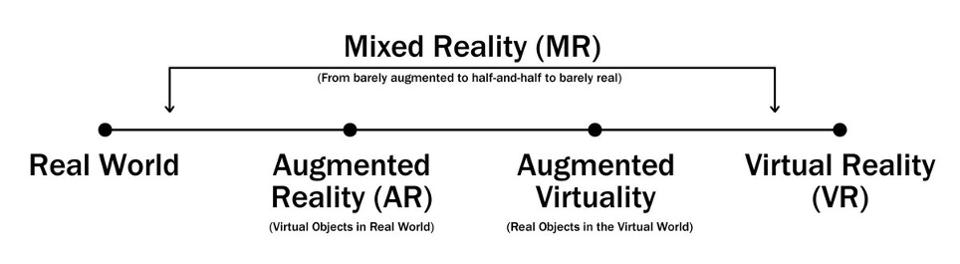
\includegraphics[scale=0.7]{images/RealitySpectrum}
\caption{Représentation de continuum de la virtualité par Milgram et Kishino, 1994.}
\label{fig:realityspectrum}
\end{figure}

\begin{figure}
\centering
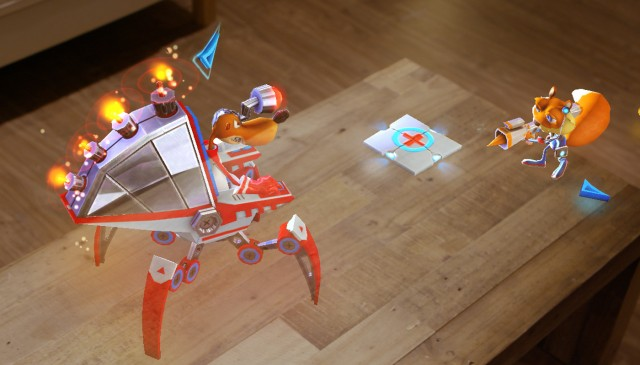
\includegraphics[scale=0.4]{images/youngconker}
\caption{Asobo Studio\texttrademark - Young Conker\copyright}
\label{fig:youngconker}
\end{figure}

\paragraph{Realité augmentée vue au travers}
La réalité augmentée vue au travers, plus communément appelé \emph{See Through Augmented Reality (STAR)} est une technique de visualisation de la réalité augmentée ou les éléments numériques sont visualisés au travers d'un écran voir Figure ~\ref{fig:STAR}

\begin{figure}[]
    \centering
	\subfloat[Pokémon GO - Vue au travers téléphone]{
      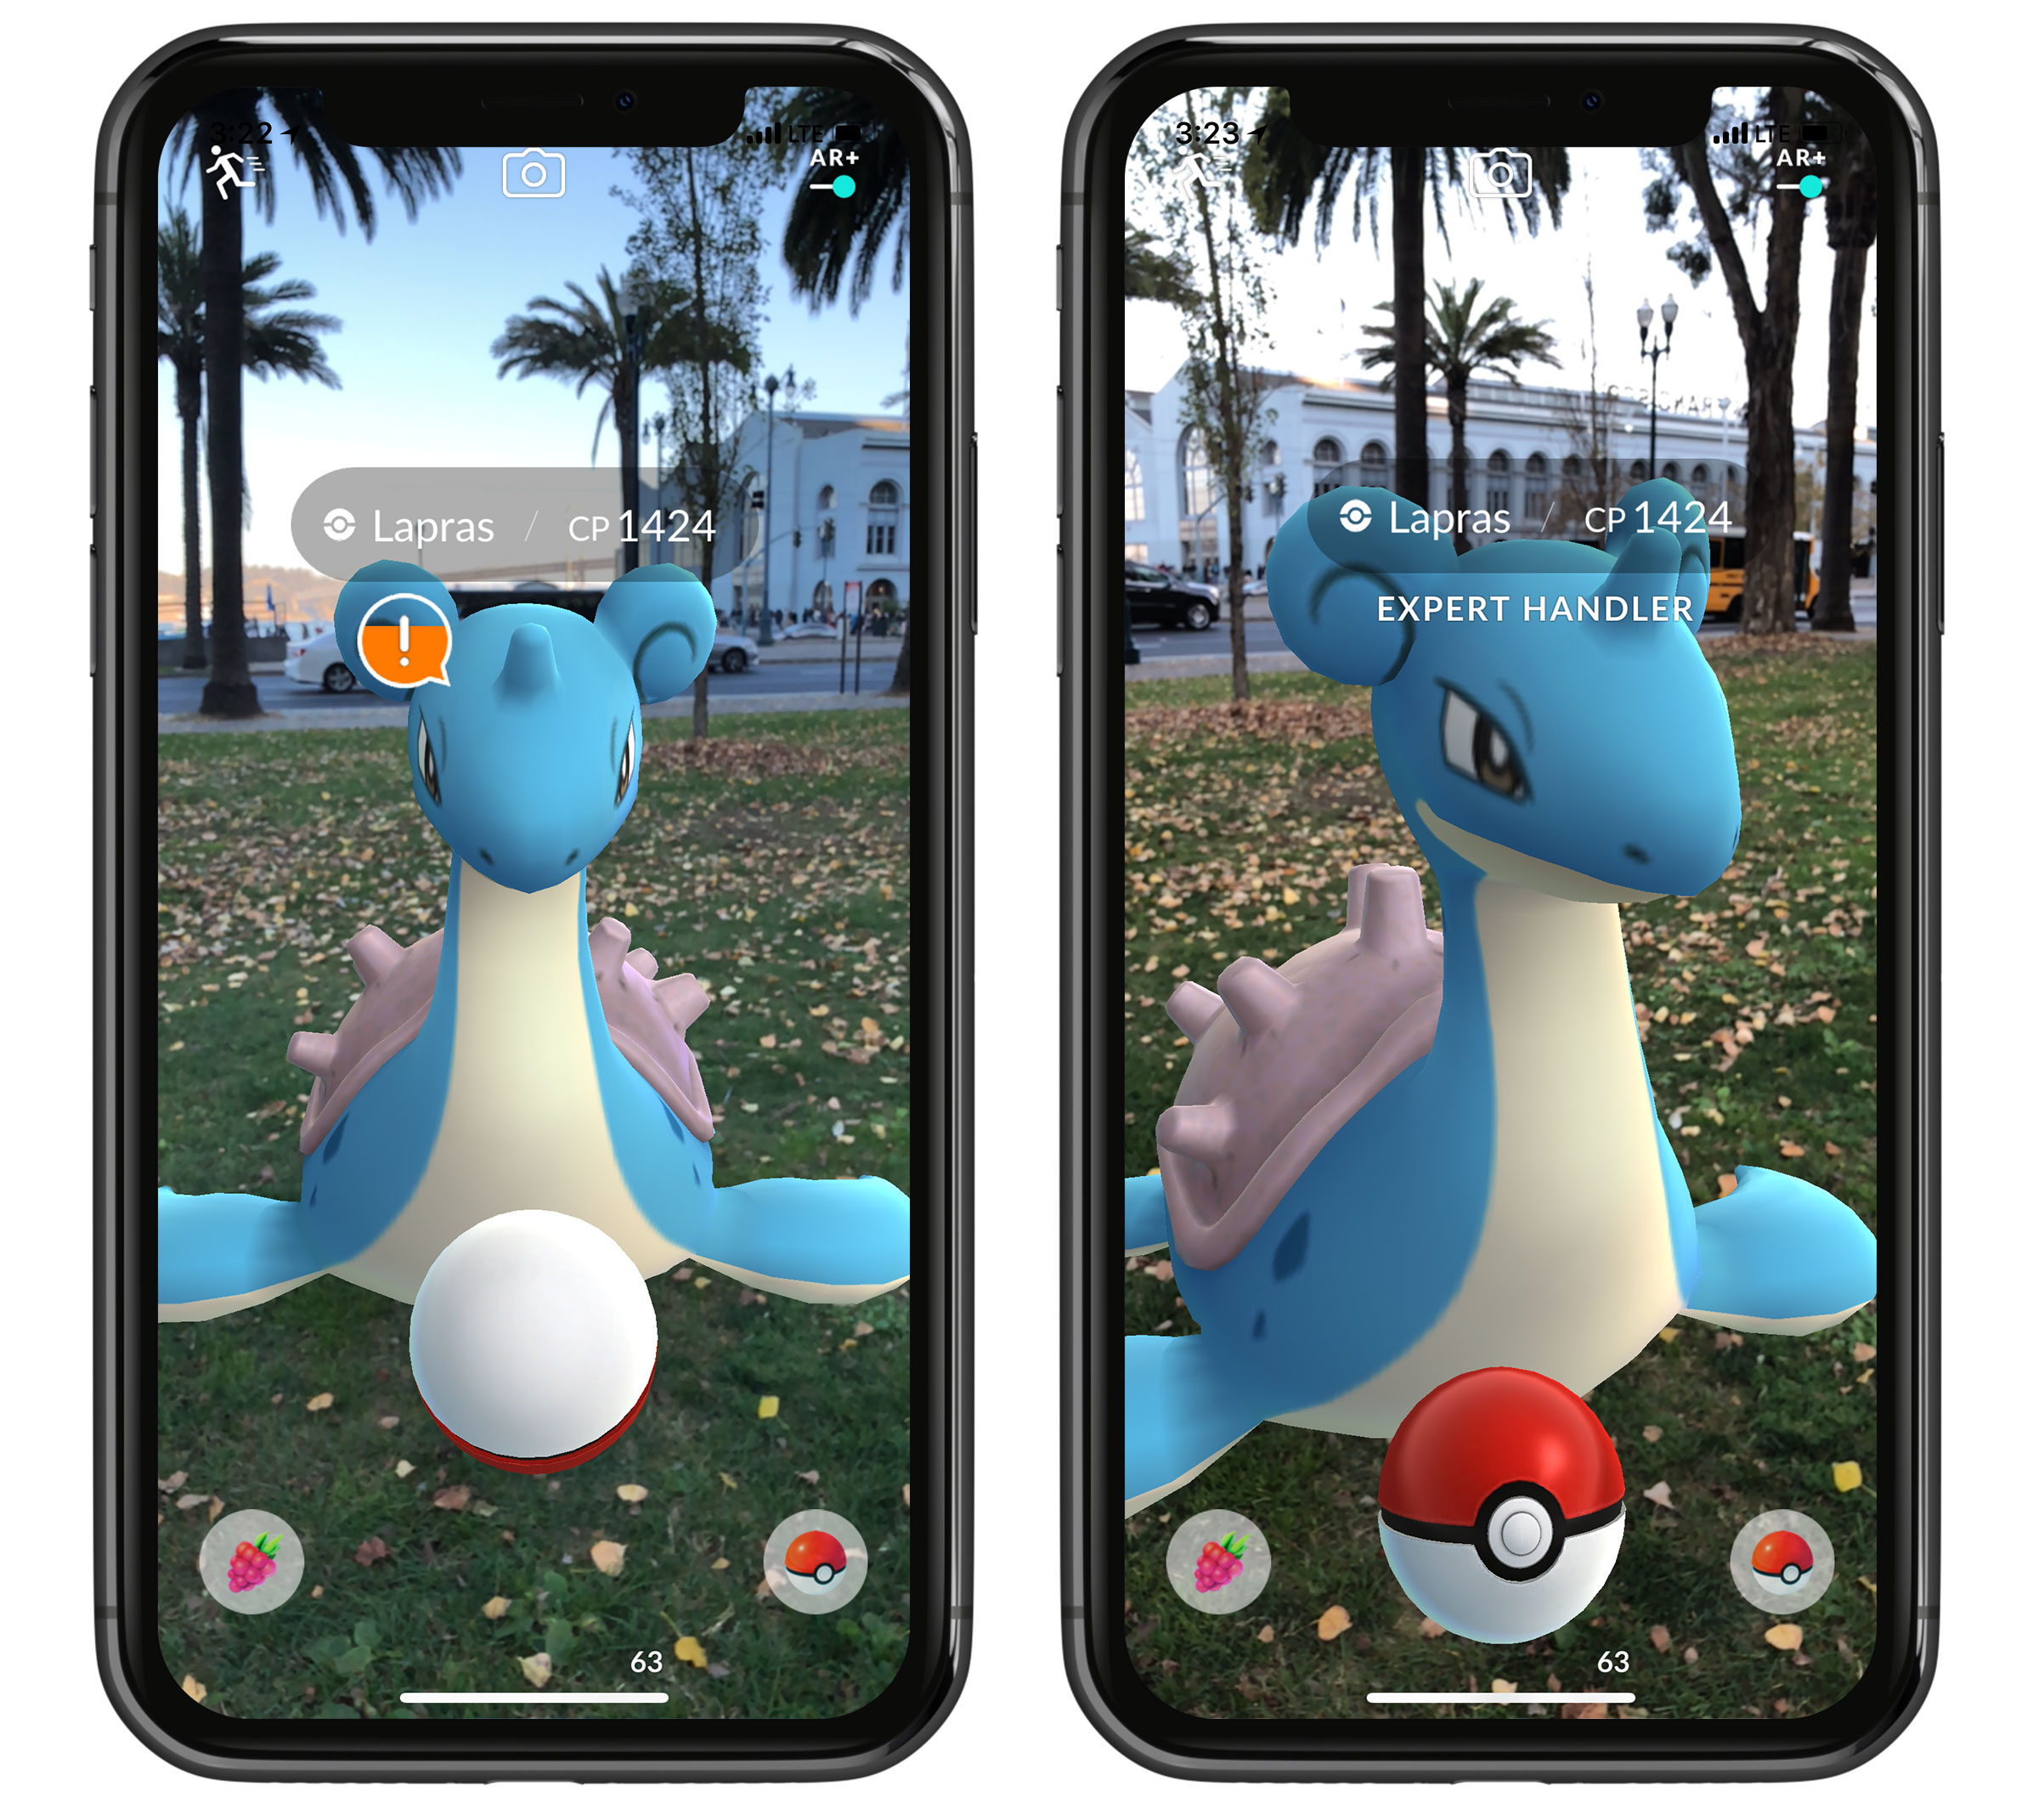
\includegraphics[width=0.45\textwidth]{images/pokemongo}
      \label{sub:STARGO}
      }
    \subfloat[Microsoft HoloLens - Vue au travers casque]{
      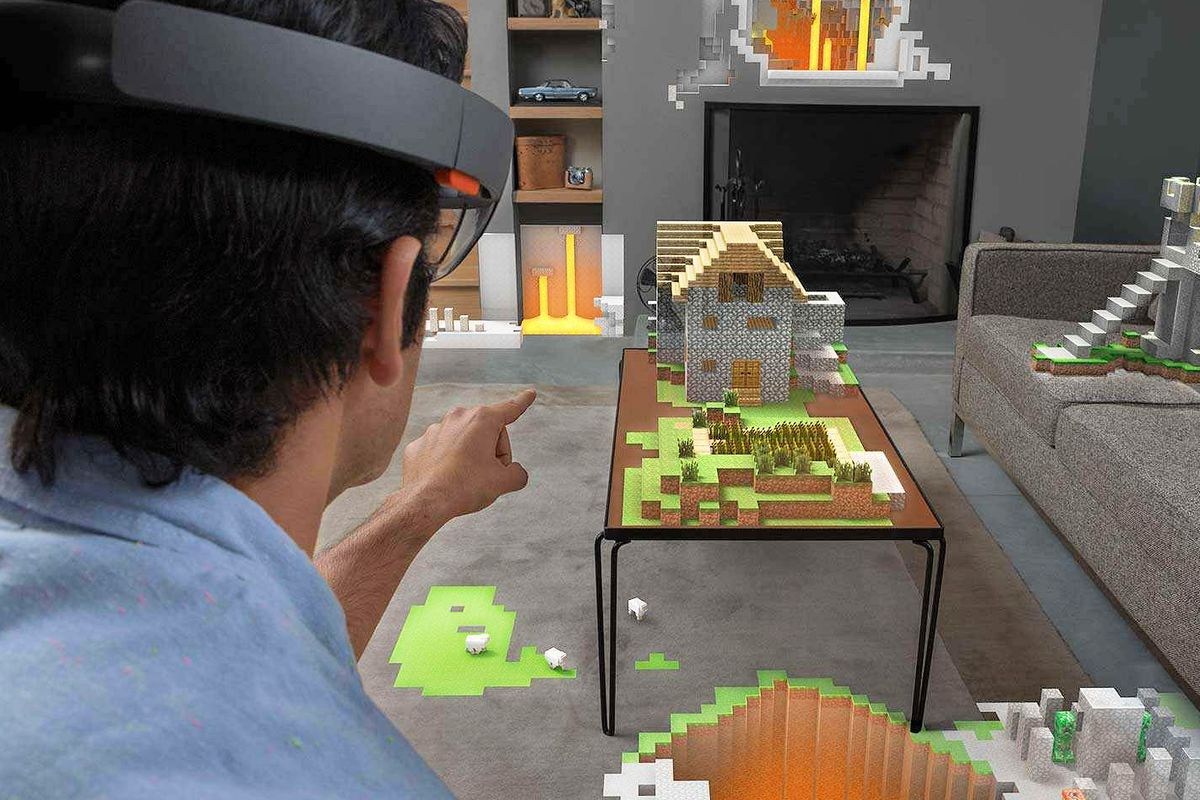
\includegraphics[width=0.45\textwidth]{images/hololens}
      \label{sub:STARHolo}
      }
\caption{Réalité augmentée vue au travers}
\label{fig:STAR}
\end{figure}


\paragraph{Réalité augmentée spatiale}
La réalité augmentée spatiale, plus communément appelé \emph{Spatial Augmented Reality (SAR)} 
\paragraph{Interfaces tangible}

\paragraph{Programmation graphique haute performance}
